%% Exemplo de utilizacao do estilo de formatacao normas-utf-tex (http://normas-utf-tex.sourceforge.net)
%% Autores: Hugo Vieira Neto (hvieir@utfpr.edu.br)
%%          Diogo Rosa Kuiaski (diogo.kuiaski@gmail.com)
%% Colaboradores:
%%          Cézar M. Vargas Benitez <cesarvargasb@gmail.com>
%%          Marcos Talau <talau@users.sourceforge.net>


\documentclass[openright]{normas-utf-tex} %openright = o capitulo comeca sempre em paginas impares
%\documentclass[oneside]{normas-utf-tex} %oneside = para dissertacoes com numero de paginas menor que 100 (apenas frente da folha) 

\usepackage[breaklinks=true]{hyperref}
\usepackage[a-3b]{pdfx}   % for PDF/A-3b

\usepackage[alf,abnt-emphasize=bf,bibjustif,recuo=0cm, abnt-etal-cite=3, abnt-etal-list=99]{abntcite} %configuracao correta das referencias bibliograficas.

\usepackage[brazil]{babel} % pacote portugues brasileiro
\usepackage[utf8]{inputenc} % pacote para acentuacao direta
\usepackage[T1]{fontenc} % pacote para  não zicar a acentuação quando copiar o texto do pdf
\usepackage{amsmath,amsfonts,amssymb} % pacote matematico
\usepackage{graphicx} % pacote grafico
%\usepackage{times} % fonte times
\usepackage{quoting}
\usepackage[none]{hyphenat}
\usepackage{microtype}
\usepackage[final]{pdfpages}

%Corrige posicionamento de figuras e tabelas quando não tem texto na página
\makeatletter
\setlength{\@fptop}{0pt}
\makeatother

%Podem utilizar GEOMETRY{...} para realizar pequenos ajustes das margens. Onde, left=esquerda, right=direita, top=superior, bottom=inferior. P.ex.:
%\geometry{left=3.0cm,right=1.5cm,top=4cm,bottom=1cm} 

% ---------- Preambulo ----------
\instituicao{Universidade Tecnológica Federal do Paraná} % nome da instituicao
\programa{Coordenadoria do Curso de Engenharia de Software} % nome do curso
\area{} % Em branco

\documento{Projeto de TCC 1} % [Projeto de TCC 1] ou [Trabalho de Conclusão de Curso] para TCC 2
\nivel{Bacharelado}
\titulacao{Bacharel}

\titulo{\MakeUppercase{Plataforma de gerenciamento de Amostras Laboratoriais e análises no Contexto do NAPI Abelhas}}
\title{Laboratory Sample and Analysis Management Platform in the Context of NAPI Abelhas}

\autor{ITALO KAIQUE BERTINI BUENO} % autor do trabalho
\cita{BUENO, Italo} % sobrenome (maiusculas), nome do autor do trabalho

% AJUSTE: Palavras-chave alinhadas ao projeto (removido "...")
\palavraschave{Apicultura. Meliponicultura. Rastreabilidade. Engenharia de Software. API REST. Docker.}
\keywords{Apiculture. Meliponiculture. Traceability. Software Engineering. REST API. Docker.} % AJUSTE: Keywords

\comentario{\UTFPRdocumentodata apresentado como requisito parcial para obtenção do título de \UTFPRtitulacaodata\ em Engenharia de Software da \ABNTinstituicaodata\ (UTFPR).}

\orientador{Prof. André Roberto Ortonceli} % nome do orientador do trabalho
%\orientador[Orientadora:]{Nome da Orientadora} % <- no caso de orientadora, usar esta sintaxe
%\coorientador[Coorientadora:]{Nome da Coorientadora} % <- no caso de coorientadora, usar esta sintaxe
%\coorientador[Coorientadores:]{Nome do Coorientador} % no caso de 2 coorientadores, usar esta sintaxe
%\coorientadorb{Nome do Co-orientador 2}	% este comando inclui o nome do 2o coorientador

\local{Dois Vizinhos} % cidade
\data{\the\year} % ano automatico

%Definir a licença do curso com as seguintes opções (deixar em branco quando não houver):
\licenca{by}

%---------- Inicio do Documento ----------
\begin{document}

\capa % geracao automatica da capa
\folhaderosto % geracao automatica da folha de rosto
%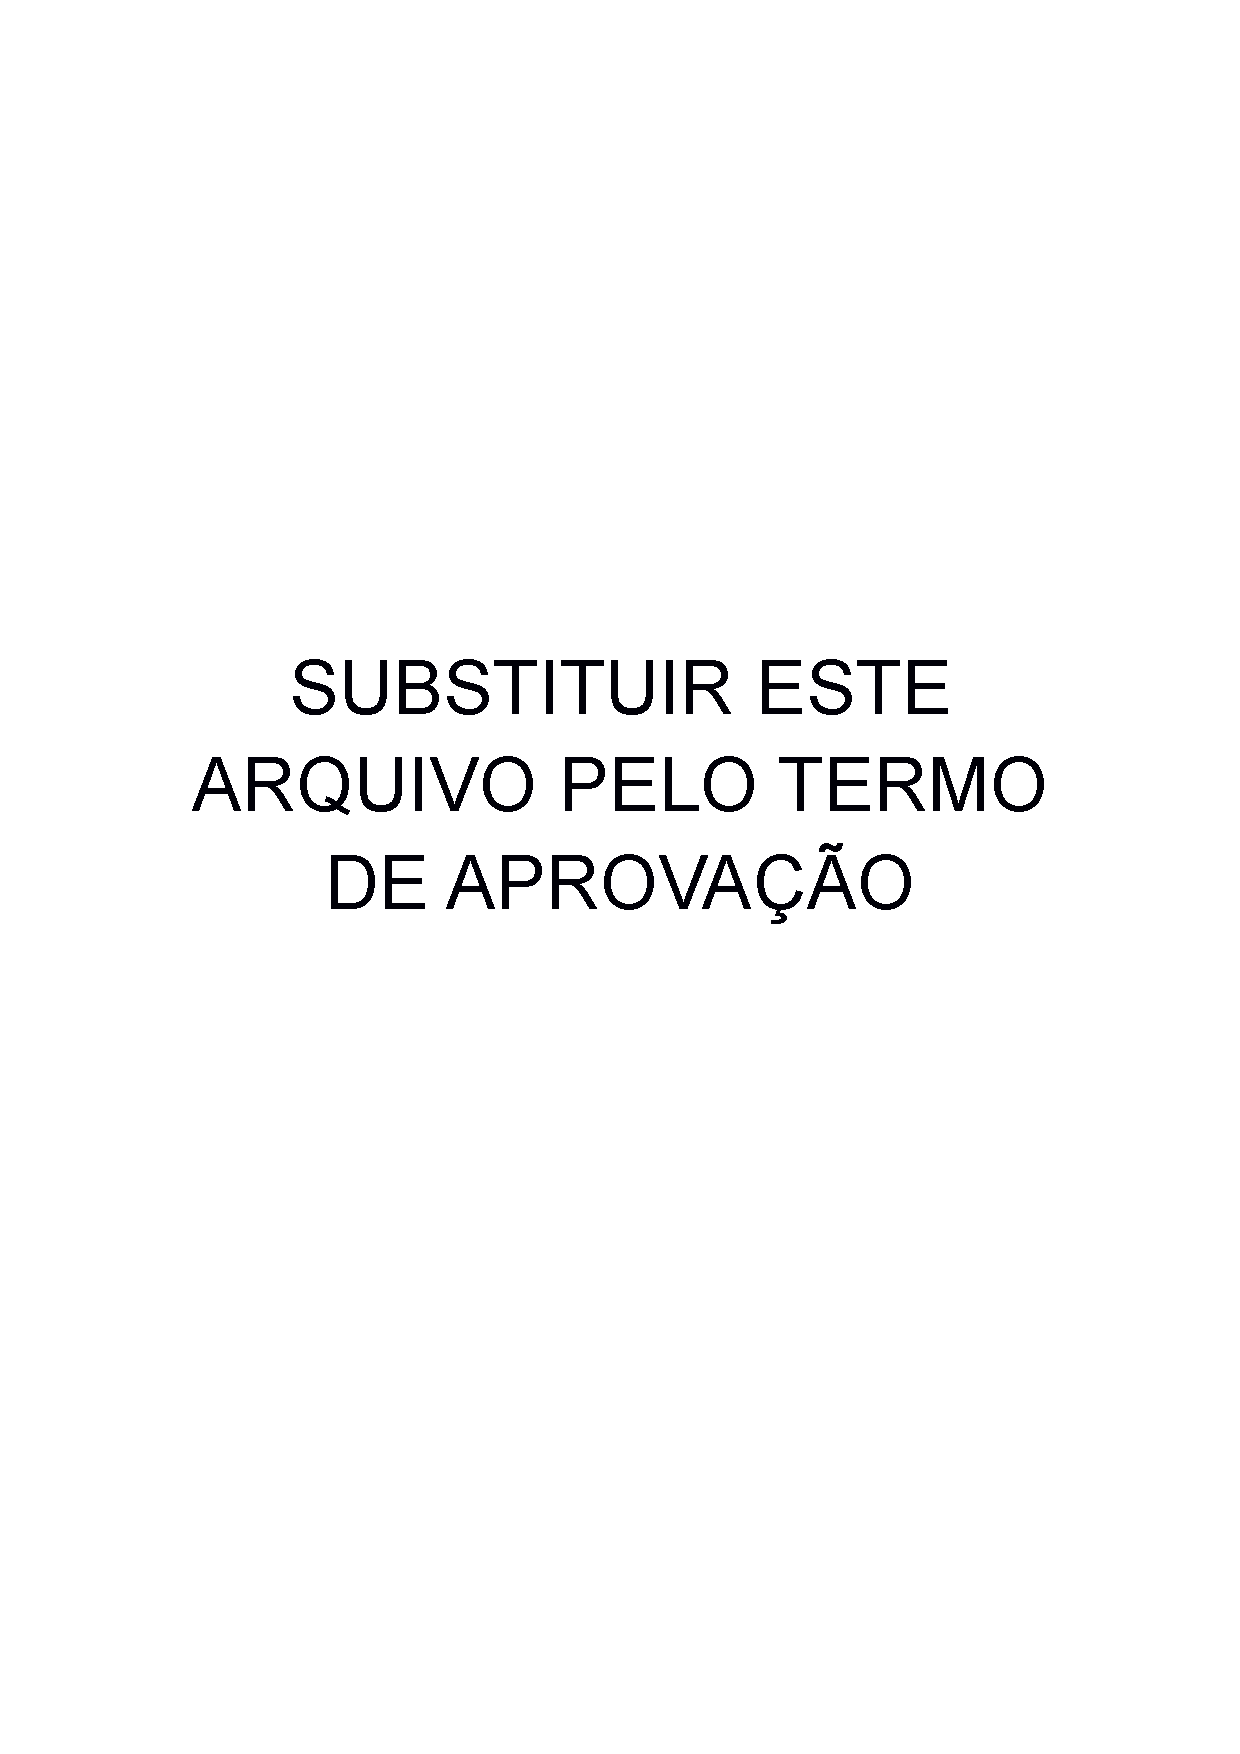
\includepdf{TermoAprovacao.pdf} Termo de Aprovação - o arquivo TermoAprovacao.pdf deve ser substituído pelo fornecido pelo Professor Responsável pelo TCC

% dedicatória (opcional)
\begin{dedicatoria}
A mim mesmo.
\end{dedicatoria}

% agradecimentos (opcional)
\begin{agradecimentos}
Agradeço ao meu orientador e a todos os demais que me auxiliaram nesta jornada.
Agradeço a minha familia
Agradeço a meus amigos.
Agradeço a minha namorada.
\end{agradecimentos}

% epigrafe (opcional)
\begin{epigrafe}
A vingança nunca é plena, mata a alma e a envenena.

Madruga, Seu.
\end{epigrafe}

% AJUSTE: Resumo focado na PROPOSTA (TCC 1), e não no TCC 2
\begin{resumo}
A gestão de amostras na apicultura e meliponicultura brasileira sofre com a descentralização e o uso de métodos manuais, como planilhas, dificultando a rastreabilidade e o controle de qualidade. Este trabalho (Projeto de TCC 1) propõe a arquitetura de uma plataforma web robusta para o gerenciamento centralizado do ciclo de vida destas amostras. A solução é baseada em uma arquitetura de serviços desacoplados, compreendendo uma API RESTful (Node.js/Express) com validação (Zod), autenticação via Clerk, armazenamento de objetos (MinIO) e cache de alta performance (Redis), consumida por uma interface web (React). O projeto detalha a modelagem do banco de dados relacional (PostgreSQL/Prisma) e a prototipagem do ambiente de desenvolvimento (Docker), visando otimizar o controle laboratorial e garantir a integridade dos dados para análises futuras.
\end{resumo}

% AJUSTE: Abstract traduzido do Resumo acima
\begin{abstract}
Sample management in Brazilian apiculture and meliponiculture suffers from decentralization and the use of manual methods, such as spreadsheets, hindering traceability and quality control. This work (TCC 1 Project) proposes the architecture for a robust web platform for the centralized management of the lifecycle of these samples. The solution is based on a decoupled services architecture, comprising a RESTful API (Node.js/Express) with validation (Zod), authentication via Clerk, object storage (MinIO), and high-performance cache (Redis), consumed by a web interface (React). The project details the relational database modeling (PostgreSQL/Prisma) and the development environment prototyping (Docker), aiming to optimize laboratory control and ensure data integrity for future analysis.
\end{abstract}

% listas (opcionais, mas recomenda-se a partir de 5 elementos)
\listadefiguras % geracao automatica da lista de figuras
\listadetabelas % geracao automatica da lista de tabelas
\listadequadros % geracao automatica da lista de quadros
\listadesiglas % geracao automatica da lista de siglas
\listadesimbolos % geracao automatica da lista de simbolos

% sumario
\sumario % geracao automatica do sumario


%---------- Inicio do Texto ----------
% recomenda-se a escrita de cada capitulo em um arquivo texto separado (exemplo: intro.tex, fund.tex, exper.tex, concl.tex, etc.) e a posterior inclusao dos mesmos no mestre do documento utilizando o comando \include{}, da seguinte forma:

\chapter{Introdução}
\label{chap:introducao}

A produção de mel e de outros produtos apícolas integra a atividade agropecuária brasileira \cite{ibge2024}. No contexto da pesquisa, a identificação da origem de uma amostra e sua associação aos resultados laboratoriais são necessárias para que os dados possam ser recuperados e interpretados posteriormente. A rastreabilidade pressupõe a possibilidade de acompanhar um produto e suas informações ao longo das etapas relevantes da cadeia \cite{iso22005}. Sistemas de informação laboratoriais oferecem uma forma de organizar esses registros \cite{gibbon1996}.

O NAPI Abelhas reúne pesquisadores de diferentes áreas e instituições no Paraná. O projeto apresentado no TCC 1 partiu da necessidade de organizar informações sobre produtores, locais de coleta, amostras e análises que estavam distribuídas em planilhas. A proposta definiu uma plataforma web e uma arquitetura inicial. O presente trabalho relata a implementação dessa plataforma, as escolhas efetivamente incorporadas aos projetos de software e as diferenças observadas em relação ao planejamento.

\section{Problema e objetivos}
\label{sec:objetivos}

O problema abordado é a fragmentação dos registros de amostras e resultados de análises, que dificulta associar cada resultado à sua origem e recuperar as informações para consultas posteriores. O objetivo geral deste trabalho é implementar e documentar uma plataforma web para o gerenciamento desses registros no contexto do NAPI Abelhas.

Os objetivos específicos são:
\begin{itemize}
    \item modelar produtores, pontos de coleta, espécies de abelhas, tipos de amostra, amostras, análises e arquivos associados;
    \item implementar uma interface de cadastro e consulta e uma API para persistência e recuperação dos dados;
    \item integrar autenticação e controle de acesso por organização e papel;
    \item disponibilizar o envio e a recuperação de arquivos associados às análises;
    \item comparar a implementação com os requisitos do TCC 1 e registrar as limitações constatadas.
\end{itemize}

\section{Procedimentos adotados}
\label{sec:metodologia}

O trabalho tem caráter aplicado: parte de uma proposta de sistema e apresenta seus artefatos de implementação. A descrição técnica foi construída por inspeção do código-fonte do frontend, da API, do esquema Prisma e da configuração de infraestrutura. A comparação com o TCC 1 considera uma funcionalidade implementada apenas quando há evidência correspondente nesses artefatos. A presença de uma tecnologia no arquivo de dependências ou na configuração de contêineres, isoladamente, não demonstra que a funcionalidade planejada esteja em operação.

A verificação descrita no Capítulo \ref{chap:resultados} separa a inspeção estática, os testes automatizados disponíveis e as capturas de interface previstas. Não houve estudo de usabilidade, entrevista ou validação com pesquisadores e técnicos do NAPI Abelhas. Consequentemente, o texto não atribui à plataforma ganhos mensurados de produtividade, desempenho ou qualidade dos dados.

\section{Organização do trabalho}

O Capítulo \ref{chap:sistema_implementado} apresenta requisitos, atividades de desenvolvimento, arquitetura e persistência, indicando as alterações de escopo observadas. O Capítulo \ref{chap:resultados} reúne as funcionalidades identificadas, as evidências técnicas e as limitações. O Capítulo \ref{chap:conclusao} sintetiza as contribuições e indica trabalhos futuros.

\chapter{Sistema Proposto}
\label{chap:sistema_proposto}

A solução proposta visa anteder inicialmente os membros NAPI Abelhas, podendo em etapa futura atender outros grupos de pesquisadores do Brasil e do Mundo, de diferentes instituições. Será necessário registrar dados de pesquisadores, produtores e técnicos responsáveis por cada amostra, mas como usuário do sistema, na sua versão proposta neste documento, irá existir apenas um perfil de usuário administrador, referente a função do técnico responsável.

A solução foi projetada para atender uma das principais demandas dos pesquisadores do NAPI Abelhas, focando na integridade dos dados, na rastreabilidade e na eficiência do fluxo de trabalho. A seguir, são detalhados os requisitos e a arquitetura do sistema.

\section{Requisitos}
\label{sec:requisitos}

\subsection{Requisitos Funcionais}

As funcionalidades do sistema foram estruturadas em módulos lógicos para cobrir o fluxo operacional do laboratório e as necessidades administrativas do NAPI Abelhas.

\begin{itemize}
    \item \textbf{Módulo de Gestão Administrativa:}
    \begin{itemize}
        \item \textbf{Controle de Acesso e Identidade:}  O sistema garante que apenas usuários autorizados (Responsáveis Técnicos) acessem as funcionalidades de escrita, mantendo um registro auditável de quem realizou cada operação (vínculo com a entidade \textit{Responsável}).
        Integração com o serviço externo \textit{Clerk}\footnote{Uma plataforma autenticação e gerenciamento de usuário: https://clerk.com/} para autenticação segura.
        
        \item \textbf{Gestão de Produtores e Pontos de Coleta:} Funcionalidade de cadastro completo de apicultores e meliponicultores. Inclui o registro georreferenciado (latitude, longitude e raio) dos apiários (\textit{ponto de coleta} das amostras), permitindo a correlação futura entre informações obtidas das amostras e suas respectiva região de origem, viabilizando a execução de pesquisas relacionadas a certificação de origem geográfica do mel produzido e identificação de condições atípicas/sazonais, que impactam na produção do mel em micro e macro regiões.
    \end{itemize}
    
    \item \textbf{Módulo para Gestão das Amostras e Análises:}
    \begin{itemize}
        \item \textbf{Recepção e Rastreabilidade (Check-in):} Processo de digitalização da entrada da amostra física produzidas pelo NAPI. O sistema gera um identificador único (UUID) para a entidade \textit{Amostra}, vinculando-a obrigatoriamente a um produtor, a um ponto de coleta, a uma espécie de abelha, a um tipo de amostra e a imagens relacionadas, e ao local onde essas amostras estão armazenadas, estabelecendo a base para a rastreabilidade total.
        \item \textbf{Gerenciamento de Análises:} Interface para a criação e acompanhamento de das análises físico-químicas realizadas. O sistema permite atribuir múltiplos tipos de exames vinculados a cada amostra, sendo que para cada um diferente tipo de arquivo com seus resultados serão armazenados no sistema. Será utilizado um padrão de \textit{Pre-signed URLs} para realizar uploads diretos e seguros para o \textit{Object Storage} (MinIO), garantindo que documentos pesados não impactem a performance da API.
    \end{itemize}
    \item \textbf{Módulo de Consultas:}
    \begin{itemize}
        %\item \textbf{Gestão Documental (Upload Seguro):} Mecanismo para envio de arquivos de laudos e evidências visuais.
        \item \textbf{Consultas com filtros:} deve ser possível consultar os dados cadastrados, com filtros relacionados ao produto, tipo de amostra, período, status, entre outros.
        
         %Ferramenta de busca avançada que permite localizar amostras por produtor, período ou status. Facilita a recuperação de laudos antigos armazenados na tabela \textit{File}, servindo como repositório centralizado de informações do NAPI.
    \end{itemize}
\end{itemize}

\subsection{Requisitos Não-Funcionais}

Os requisitos não-funcionais definem os atributos de qualidade e as restrições técnicas da solução proposta:

\begin{itemize}
    \item \textbf{Segurança:} para garantir um acesso seguro aos dados, a aplicação proposta não irá armazenar senhas localmente, delegando a autenticação ao uso de tokens JWT. O acesso aos arquivos de laudos será protegido por URLs assinadas temporárias, com tempo de expiração reduzido para visualização.

    \item \textbf{Desempenho (Performance):} com o crescimento progressivo do número de usuários — envolvendo inicialmente pesquisadores de todo o estado — o sistema deve apresentar desempenho capaz de suportar um aumento de acessos a médio prazo. Para isso, o sistema proposto utilizará uma estratégia \textit{Cache-First} (Redis) para dados de leitura frequente e baixa volatilidade (como listas de cidades, espécies de abelhas e tipos de análise), reduzindo a latência da interface.

    \item \textbf{Escalabilidade e Portabilidade:} existe a necessidade de que a aplicação possa ser implantada, atualizada e ampliada de maneira eficiente, acompanhando o aumento da demanda e possíveis mudanças de infraestrutura. Para tal, a arquitetura será integralmente baseada em contêineres (Docker), permitindo que a API, o banco de dados e os serviços de suporte sejam implantados e escalados de forma independente em qualquer ambiente compatível.

\end{itemize}


\section{Tecnologias Utilizadas}
\label{sec:tecnologias}

A seleção tecnológica priorizou ferramentas de código aberto, robustas e amplamente adotadas pelo mercado, visando atender aos requisitos de desempenho e escalabilidade do projeto.

\begin{itemize}
    \item \textbf{Linguagem e Runtime:}
        \begin{itemize}
            \item \textbf{Node.js:} Ambiente de execução JavaScript assíncrono e orientado a eventos, construído sobre o motor V8 do Google Chrome, ideal para aplicações escaláveis de rede \cite{casciaro2020}.
            \item \textbf{TypeScript:} Superconjunto do JavaScript que adiciona tipagem estática opcional à linguagem, proporcionando maior segurança no desenvolvimento e facilidade na manutenção do código \cite{cherny2019}.
        \end{itemize}

    \item \textbf{Frontend:}
        \begin{itemize}
            \item \textbf{React:} Biblioteca JavaScript declarativa, eficiente e flexível para a construção de interfaces de usuário baseadas em componentes \cite{banks2020}.
            \item \textbf{Vite:} Ferramenta de construção (\textit{build tool}) que utiliza o suporte nativo a módulos ES (ESM) para oferecer um ambiente de desenvolvimento com recarregamento rápido e otimizado \cite{vite2024}.
        \end{itemize}

    \item \textbf{Persistência:}
        \begin{itemize}
            \item \textbf{PostgreSQL:} Sistema gerenciador de banco de dados objeto-relacional (ORDBMS) de código aberto, reconhecido por sua robustez, conformidade com padrões ACID e extensibilidade \cite{postgres2024}.
            \item \textbf{Prisma ORM:} Mapeador objeto-relacional moderno que oferece segurança de tipos (\textit{type-safety}) e gerencia migrações de esquema de forma declarativa \cite{prisma2024}.
        \end{itemize}

    \item \textbf{Armazenamento e Cache:}
        \begin{itemize}
            \item \textbf{MinIO:} Servidor de armazenamento de objetos de alto desempenho, compatível com a API Amazon S3, utilizado para persistência segura de arquivos não estruturados \cite{minio2024}.
            \item \textbf{Redis:} Armazenamento de estrutura de dados em memória, utilizado como banco de dados, cache e \textit{message broker} para otimização de latência \cite{redis2024}.
        \end{itemize}

    \item \textbf{Segurança e Infraestrutura:}
        \begin{itemize}
            \item \textbf{Clerk:} Solução completa de gerenciamento de identidade e acesso (IAM), fornecendo autenticação segura e gestão de sessões de usuário \cite{clerk2024}.
            \item \textbf{Docker:} Plataforma de software para desenvolvimento, envio e execução de aplicações dentro de contêineres, garantindo isolamento e portabilidade entre ambientes \cite{poulton2023}.
        \end{itemize}
\end{itemize}

\section{Arquitetura Proposta}
\label{sec:arquitetura}
A arquitetura da solução segue o modelo de serviços desacoplados, visando escalabilidade e facilidade de manutenção. A Figura \ref{fig:arquitetura} ilustra a visão geral dos componentes e suas interações.

O \textit{Frontend} (React) atua como cliente consumidor, comunicando-se com a API Backend para operações transacionais e interagindo diretamente com o \textit{Object Storage} (MinIO) para a transferência de arquivos binários, otimizando o tráfego de rede.

\begin{figure}[H]
    \centering
    \caption{Visão Geral da Arquitetura do Sistema}
    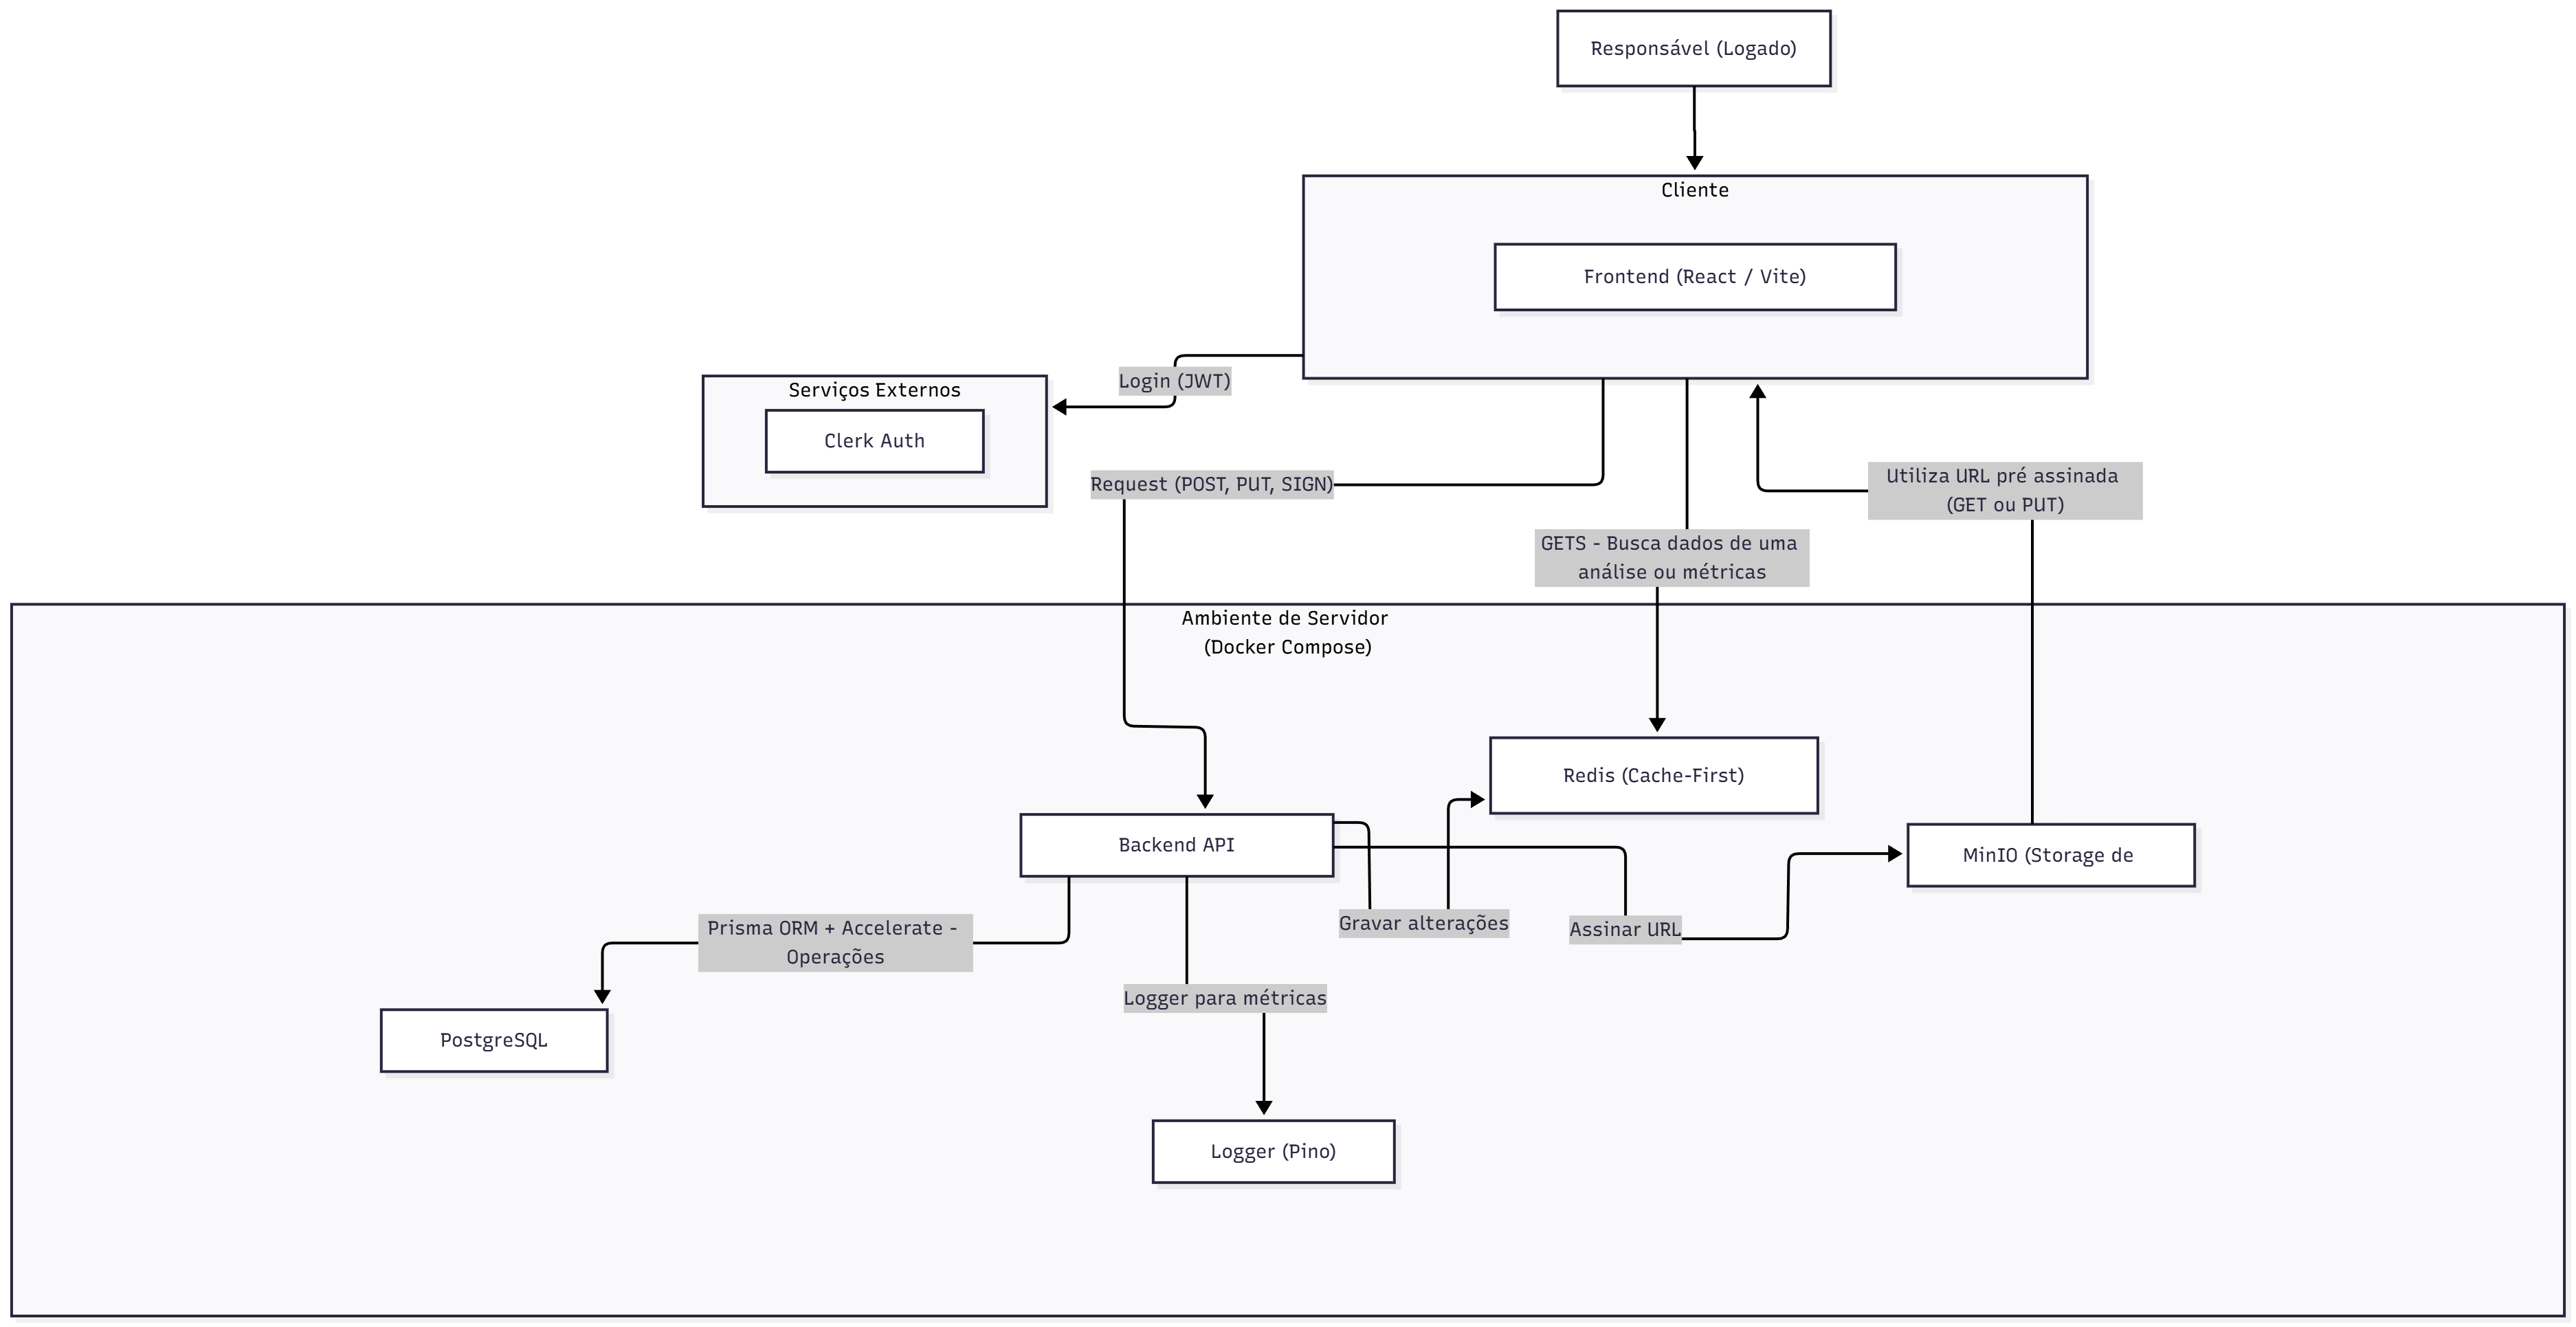
\includegraphics[width=1.0\textwidth]{Imagens/diagramaArquitetura.png}
    \fonte{Autoria própria (2025).}
    \label{fig:arquitetura}
\end{figure}

\section{Persistência de Dados}
\label{sec:persistencia}

A persistência adota uma abordagem híbrida: dados estruturados relacionais para garantir a integridade do negócio e armazenamento de objetos para arquivos binários. A Figura \ref{fig:der} apresenta o Modelo Lógico do Banco de Dados.

Entidades principais como \textit{Amostra}, \textit{Produtor} e \textit{Análise} são mantidas no PostgreSQL para garantir integridade referencial estrita, enquanto as tabelas \textit{File} e \textit{FileGroup} gerenciam apenas os metadados e ponteiros para os arquivos físicos salvos no \textit{Storage}.

\begin{figure}
    \centering
    \caption{Diagrama Entidade-Relacionamento (DER) Lógico}
    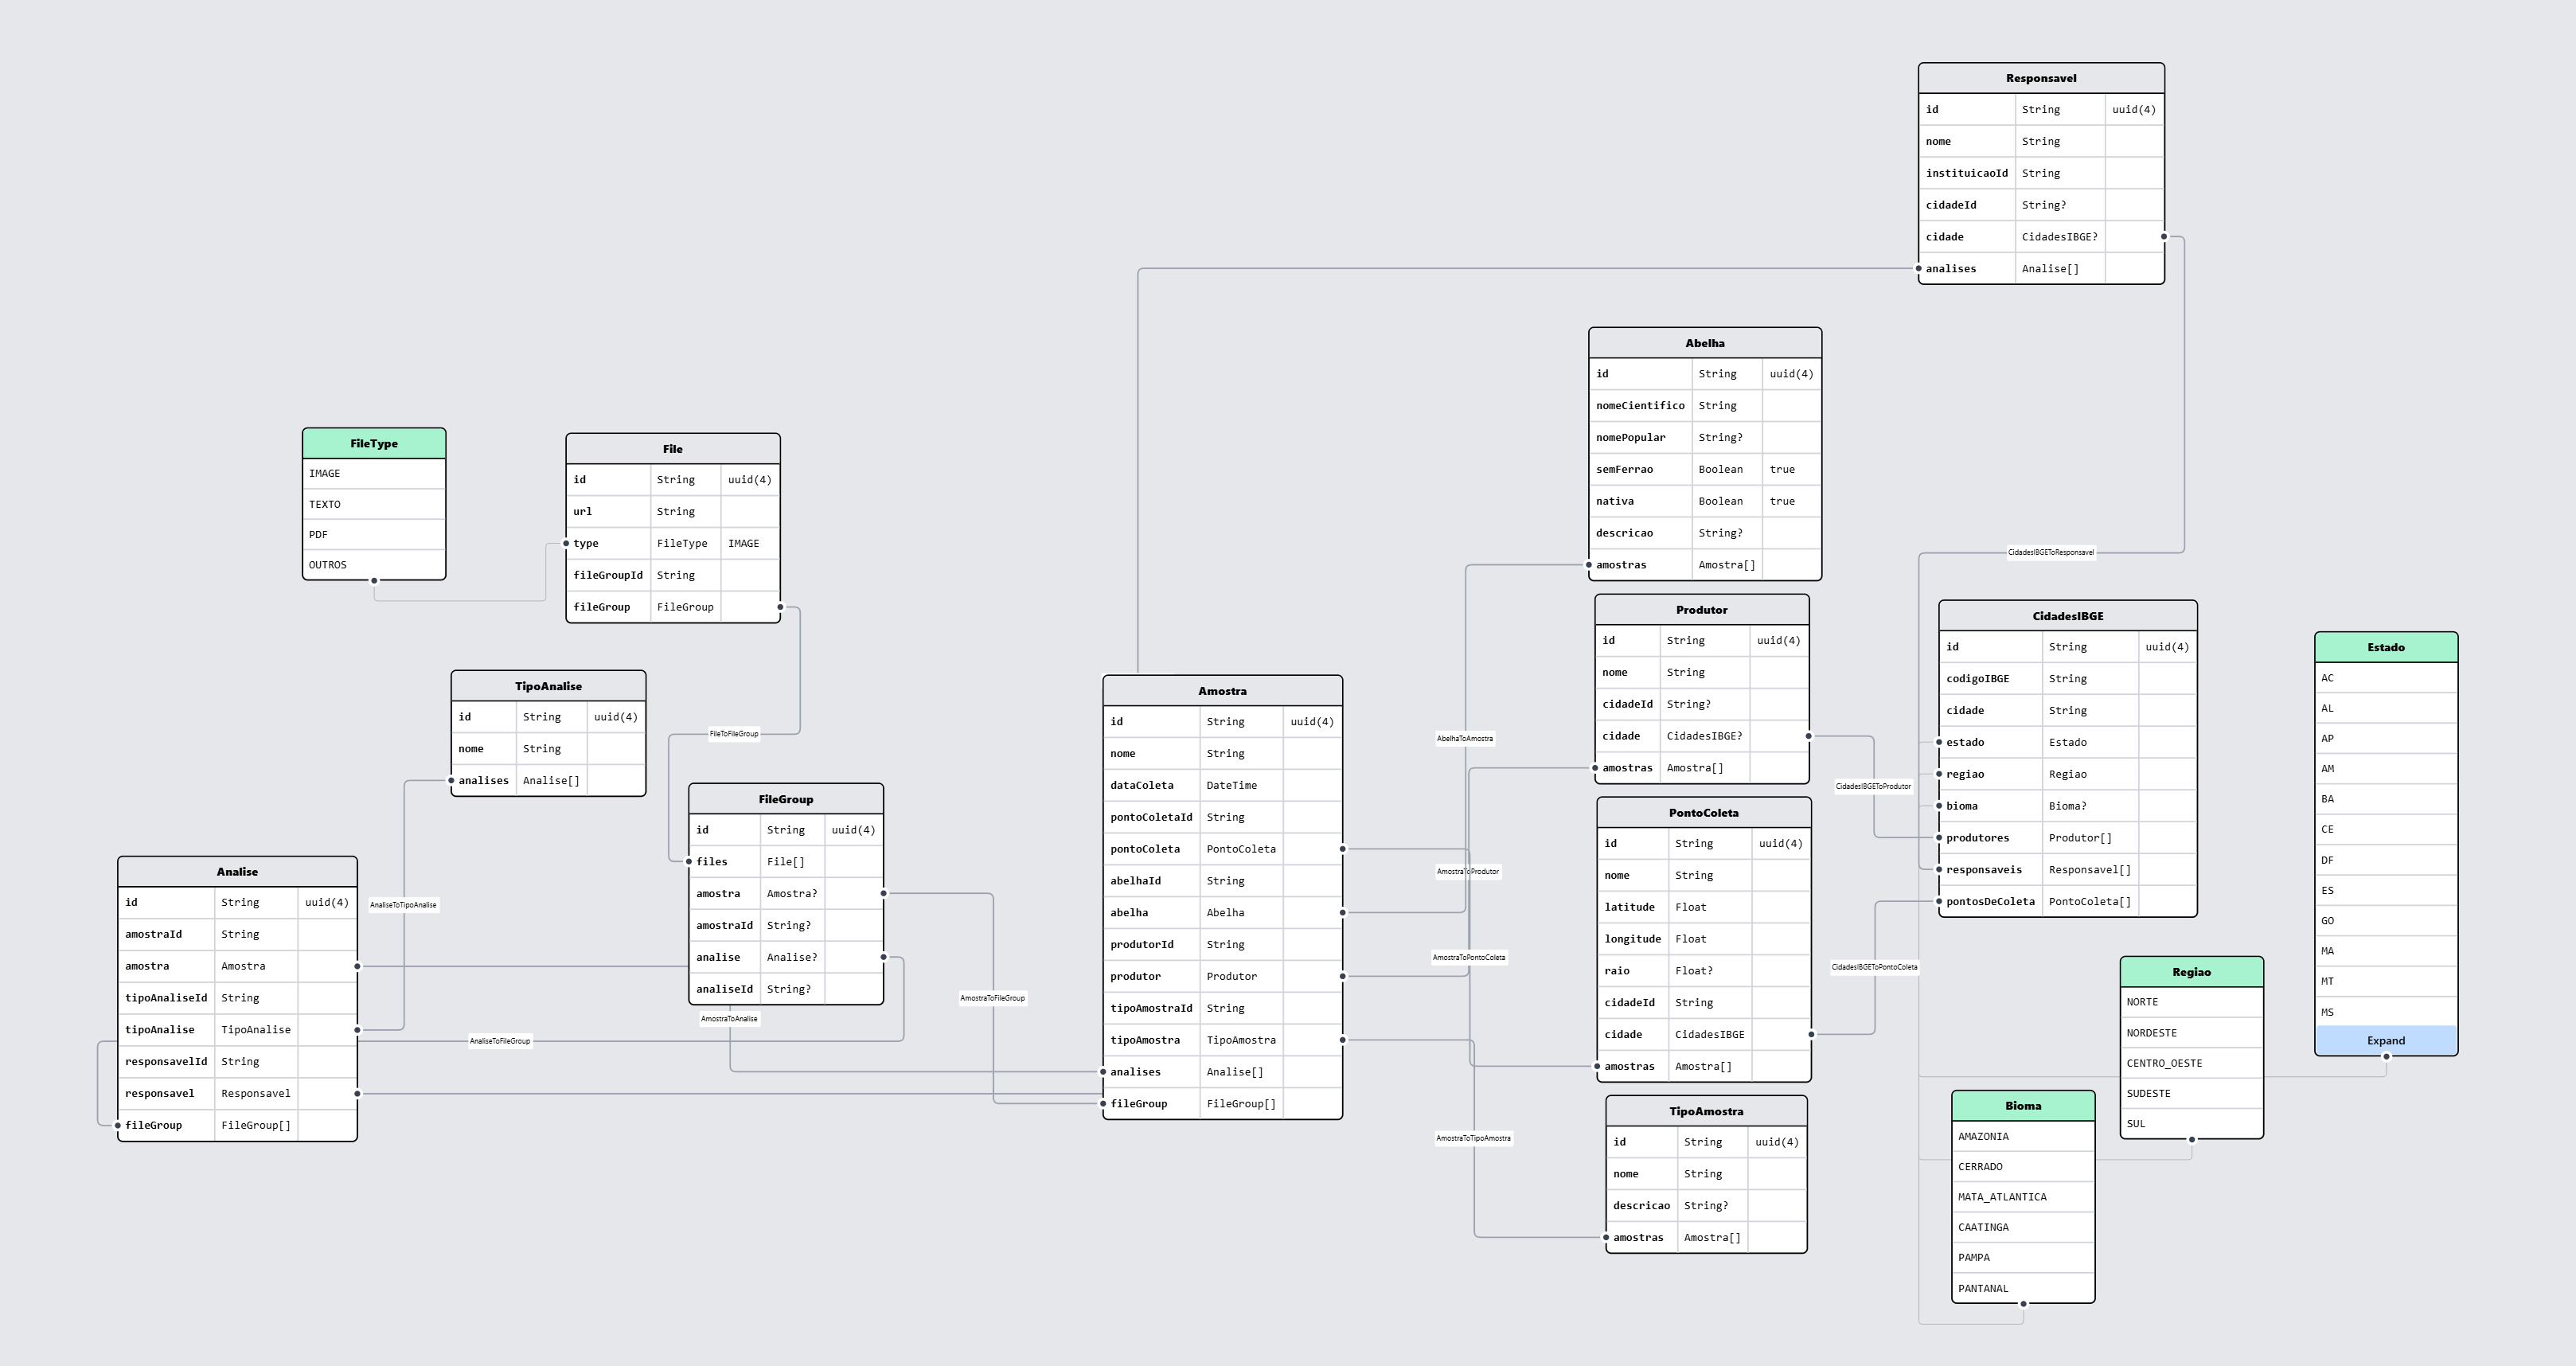
\includegraphics[width=1.0\textwidth]{Imagens/diagramaDB.png}
    \fonte{Autoria própria (2025).}
    \label{fig:der}
\end{figure}

\chapter{Cronograma de Desenvolvimento}

O desenvolvimento da Plataforma de Gerenciamento de Amostras e Análises de Abelhas será executado ao longo do próximo semestre letivo, correspondendo à disciplina de Trabalho de Conclusão de Curso 2 (TCC 2). O planejamento foi estruturado para garantir a entrega incremental de valor, seguindo os princípios ágeis adotados na metodologia.

As atividades foram divididas em fases lógicas, desde a configuração do ambiente até a validação final com usuários e defesa do trabalho.

\begin{table}[ht]
\centering
\caption{Cronograma de Atividades Previsto para o TCC 2}
\label{tab:cronograma}
\vspace{0.2cm}
\resizebox{\textwidth}{!}{% Redimensiona a tabela para caber na largura da página
\begin{tabular}{|l|c|c|c|c|c|c|}
\hline
\textbf{Atividades / Mês} & \textbf{Mês 1} & \textbf{Mês 2} & \textbf{Mês 3} & \textbf{Mês 4} & \textbf{Mês 5} & \textbf{Mês 6} \\ \hline
Revisão e Refinamento de Requisitos & X & & & & & \\ \hline
Configuração do Ambiente (Docker/CI) & X & & & & & \\ \hline
Implementação do Banco de Dados & X & X & & & & \\ \hline
Desenvolvimento do Backend (API) & & X & X & & & \\ \hline
Desenvolvimento do Frontend (React) & & & X & X & & \\ \hline
Integração e Testes Unitários & & & & X & X & \\ \hline
Escrita da Monografia Final & & X & X & X & X & \\ \hline
Revisão Final e Preparação da Defesa & & & & & & X \\ \hline
\end{tabular}%
}
\par
\vspace{0.2cm}
\small{Fonte: Autoria própria (2025).}
\end{table}

\section{Detalhamento das Etapas}

\begin{itemize}
    \item \textbf{Mês 1 (Fundação):} Foco na infraestrutura DevOps. Configuração dos containers Docker para o banco de dados PostgreSQL e o sistema de arquivos MinIO. Criação das migrações iniciais do Prisma ORM.
    \item \textbf{Mês 2 e 3 (Core Backend):} Desenvolvimento dos microsserviços principais em Node.js. Implementação da autenticação, gestão de perfis de usuário e CRUD de amostras.
    \item \textbf{Mês 4 (Frontend e Integração):} Construção das interfaces em React. Integração com a API REST. Implementação da funcionalidade de upload de laudos.
    \item \textbf{Mês 5 (Refinamento):} Testes de ponta a ponta, correção de bugs (polimento) e finalização da escrita acadêmica.
    \item \textbf{Mês 6 (Conclusão):} Entrega da versão final do documento e apresentação para a banca examinadora.
\end{itemize}

% \chapter{Recursos}

Apresente aqui todos os recursos essenciais ao desenvolvimento do projeto. O(s) aluno(s) deve(m) mencionar também a origem dos recursos (próprios, externos ou da UTFPR) e a viabilidade do projeto.

Devem ser apresentados aqui os recursos de software, incluindo os principais fundamentos (teorias, algoritmos, paradigmas) e tecnologias (ambientes de desenvolvimento, linguagens de programação) a serem empregados. Especifique a origem dos recursos de software. % Não obrigatório porém, a critério do estudante/orientador pode ser adicionado
% \chapter{Resultados}

Resultados finais do trabalho. % Não obrigatório porém, a critério do estudante/orientador pode ser adicionado
\chapter{Conclusões}
\label{chap:conclusao}

Este trabalho apresentou a implementação de uma plataforma web para organizar informações de produtores, pontos de coleta, amostras, análises e arquivos no contexto do NAPI Abelhas. A solução materializa parte central da proposta do TCC 1: associa a amostra à sua origem, mantém análises vinculadas e disponibiliza o envio de documentos por armazenamento de objetos. A interface em Next.js e a API em NestJS, com PostgreSQL, Prisma, Clerk e MinIO, constituem os artefatos técnicos entregues.

A comparação com o planejamento mostrou mudanças de tecnologia e de acesso. O frontend passou de Vite para Next.js, a API foi estruturada em NestJS sobre Express, e o perfil único previsto deu lugar a organizações com papéis de administrador e membro. Também evidenciou requisitos ainda não demonstrados: filtros avançados no servidor, registro do local físico da amostra, imagem obrigatória no cadastro e uso efetivo de Redis como cache. Assim, o resultado deve ser compreendido como uma implementação com limites identificados, e não como comprovação de atendimento integral ao escopo inicialmente proposto.

Como continuidade, recomenda-se completar os requisitos pendentes, ampliar os testes automatizados dos fluxos de negócio e executar testes de ponta a ponta em ambiente configurado com dados fictícios. Uma avaliação posterior com pesquisadores e técnicos poderá verificar a adequação dos formulários, da navegação e das consultas às rotinas reais do NAPI Abelhas. Somente com essa avaliação e com medições específicas será possível afirmar efeitos da plataforma sobre produtividade, desempenho ou qualidade das informações.



%---------- Referencias ----------
\clearpage % this is need for add +1 to pageref of bibstart used in 'ficha catalografica'.
\label{bibstart}
\bibliography{Capitulos/reflatex} % geracao automatica das referencias a partir do arquivo reflatex.bib
\label{bibend}


% --------- Lista de siglas --------
%\textbf{* Observa\c{c}\~oes:} a lista de siglas nao realiza a ordenacao das siglas em ordem alfabetica
% Em breve isso sera implementado, enquanto isso:
%\textbf{Sugest\~ao:} crie outro arquivo .tex para siglas e utilize o comando \sigla{sigla}{descri\c{c}\~ao}.
%Para incluir este arquivo no final do arquivo, utilize o comando \input{arquivo.tex}.
%Assim, Todas as siglas serao geradas na ultima pagina. Entao, devera excluir a ultima pagina da versao final do arquivo
% PDF do seu documento.


%-------- Citacoes ---------
% - Utilize o comando \citeonline{...} para citacoes com o seguinte formato: Autor et al. (2011).
% Este tipo de formato eh utilizado no comeco do paragrafo. P.ex.: \citeonline{autor2011}

% - Utilize o comando \cite{...} para citacoeses no meio ou final do paragrafo. P.ex.: \cite{autor2011}



%-------- Titulos com nomes cientificos (titulo, capitulos e secoes) ----------
% Regra para escrita de nomes cientificos:
% Os nomes devem ser escritos em italico, 
%a primeira letra do primeiro nome deve ser em maiusculo e o restante em minusculo (inclusive a primeira letra do segundo nome).
% VEJA os exemplos abaixo.
% 
% 1) voce nao quer que a secao fique com uppercase (caixa alta) automaticamente:
%\section[nouppercase]{\MakeUppercase{Estudo dos efeitos da radiacao ultravioleta C e TFD em celulas de} {\textit{Saccharomyces boulardii}}
%
% 2) por padrao os cases (maiusculas/minuscula) sao ajustados automaticamente, voce nao precisa usar makeuppercase e afins.
% \section{Introducao} % a introducao sera posta no texto como INTRODUCAO, automaticamente, como a norma indica.


\end{document}